\documentclass{beamer}

\mode <presentation>

\usepackage{algorithmic}
\usepackage{algorithm}
\usepackage{movie15}
\usepackage{graphicx}
\usepackage{subfigure}

\usetheme{DRL}

\graphicspath{{../figures/}}

\title{Vision Based Obstacle Avoidance Using Neuro-Evolution on a Differential Drive Robot in Simulation}
\author{Devin Koepl, Kevin Kemper}

\institute[Oregon State University] % (optional, but mostly needed)
{
	Dynamic Robotics Laboratory\\
	Oregon State University
}
\date[ME 537 2010] % (optional, should be abbreviation of conference name)
	{Class Conference on Learning for Control, 2010}
\subject{Neuro-Evolution for Control} 

\pgfdeclareimage[height=1cm]{university-logo}{./Oregon_State_University_logo}
\logo{\pgfuseimage{university-logo}}

\begin{document}

\frame{\titlepage}


%%%%%%%%%%%%%%%%%%%%%%%%%%%%%%%%%%%%%%%%%%%%%%%%%%%%%%%%%%%%%%%%%%%%%%%%%%%%%%%%
\section{Introduction}

	\begin{frame}{Introduction}
	\begin{columns}[l c]

		\column{0.55\textwidth}

			\begin{itemize}
			\item Traditional approaches rely on a battery of sensors
				\begin{itemize}
				\item Can be expensive
				\item Fragile 
				\end{itemize}

			\item Many platforms utilize cameras for high-level functions
				\begin{itemize}
				\item Reduce the number of components
				\end{itemize}

			\item Vision provides a rich set of data
				\begin{itemize}
				\item Hard to interpret
				\item What is an obstacle?
				\end{itemize}

			\end{itemize}


		\column{0.48\textwidth}

			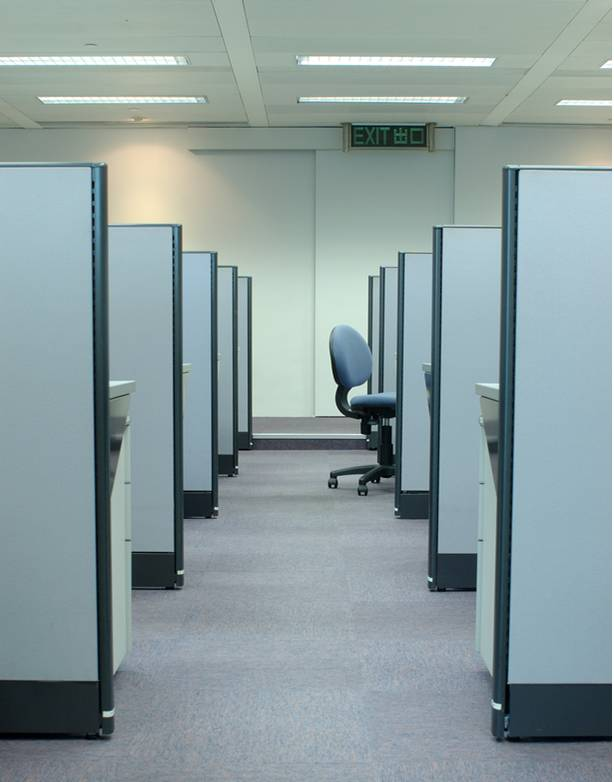
\includegraphics[width=0.4\textwidth]{cubicles.jpg}
			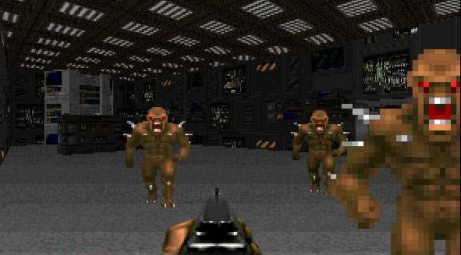
\includegraphics[width=0.6\textwidth]{doom.jpg}
			\\
			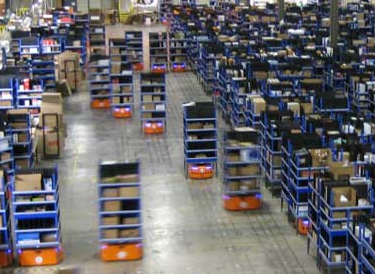
\includegraphics[width=0.5\textwidth]{kiva.png}
			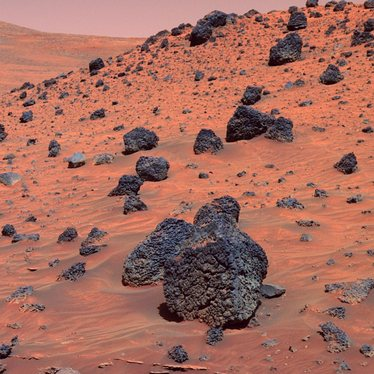
\includegraphics[width=0.5\textwidth]{mars.jpg}

	\end{columns}
	\end{frame}


%%%%%%%%%%%%%%%%%%%%%%%%%%%%%%%%%%%%%%%%%%%%%%%%%%%%%%%%%%%%%%%%%%%%%%%%%%%%%%%%
\section{Background}

	\begin{frame}{Current Vision for Control Techniques}
	\begin{columns}[l c]

		\column{0.5\textwidth}

			\begin{itemize}
			\item Optical flow
				\begin{itemize}
				\item Apparent motion of landmarks in image
				\item Requires intensive processing on several images
				\end{itemize}

			\item Neural networks
				\begin{itemize}
				\item Pixel values are inputs
				\item Learning rate slow for even moderate images
				\end{itemize}

			\end{itemize}

		\column{0.5\textwidth}

			\vspace{-24pt}
			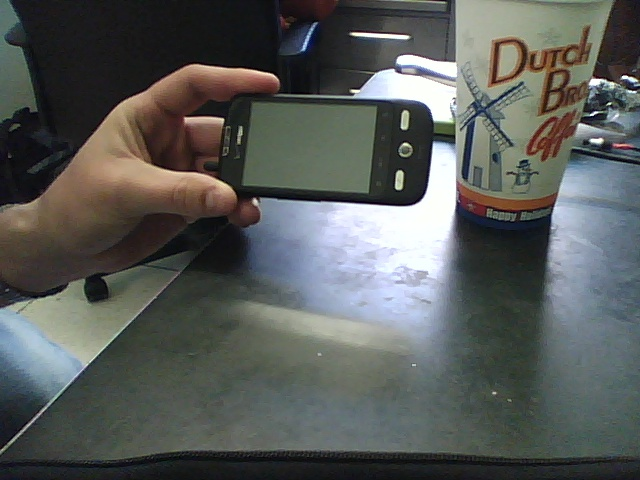
\includegraphics[width=0.5\textwidth]{input.jpg}
			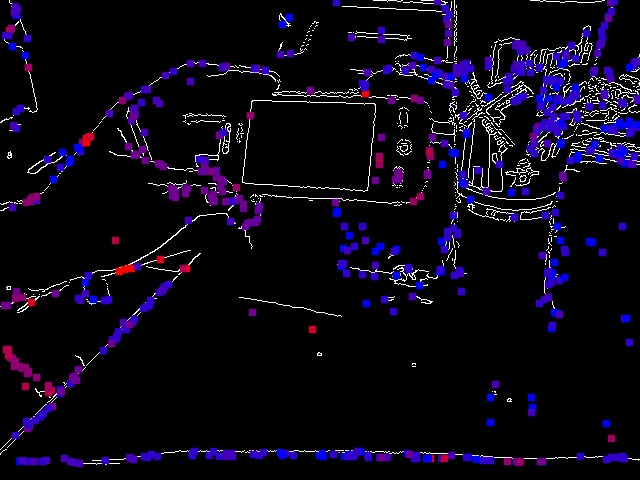
\includegraphics[width=0.5\textwidth]{output.jpg}
			\\

			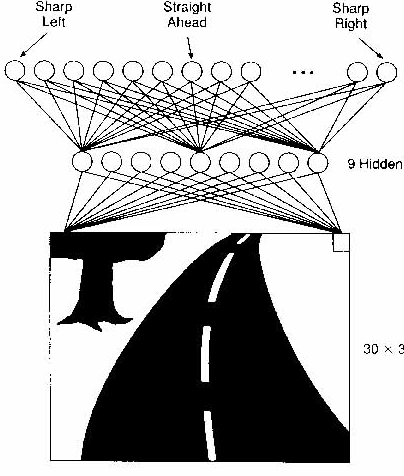
\includegraphics[width=0.5\textwidth]{alvinn.jpg}


	\end{columns}
	\end{frame}

	\begin{frame}{Ensemble Based Neuroevolution}
	\begin{columns}[l c]

	\column{0.5\textwidth}

		\begin{itemize}

		\item Robustness of ANN learning can be improved

		\item Individual errors can be taken care of %by considering the output of all ANNs in the ensemble
			\begin{itemize}
			\item Provided that ANNs make independent errors
			\end{itemize}

		\item Investigated for a variety of applications
			\begin{itemize}
			\item Pattern recognition/classification
			\item Function approximation
			\end{itemize}

		\end{itemize}



		\column{0.5\textwidth}
		
			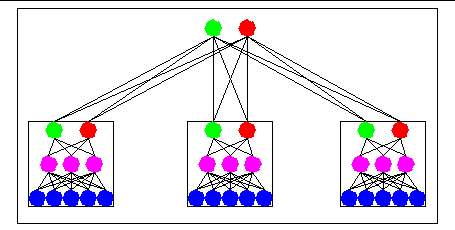
\includegraphics[width=\textwidth]{ensemble.png}

		
%			The final concept we pan to utilize revolves around ensemble methods.  It has been shown that robustness of ANN learning can be improved by ensemble methods, and considerable work has been done to investigate the potential of such methods for a variety of applications \cite{Hansen1990}.  When ANNs are grouped together in an ensemble their individual errors can be taken care of by considering the output of all ANNs in the ensemble, provided that ANNs make independent errors.  Our motivation for this work presented in this paper comes from the success of these investigations at increasing the robustness of ANN learning, provided that ANNs in an ensemble do not make identical errors, without increasing the complexity of the individual learners in the ensemble.
	\end{columns}
	\end{frame}

%%%%%%%%%%%%%%%%%%%%%%%%%%%%%%%%%%%%%%%%%%%%%%%%%%%%%%%%%%%%%%%%%%%%%%%%%%%%%%%%	
\section{Problem Domain}

	\begin{frame}{Problem Domain}

		\begin{columns}[c c]
		
			\column{0.5\textwidth}
				
				\begin{itemize}
				\item Maze Environment
					\begin{itemize}
					\item Continuous Space
					\item Realistic Physics
					\end{itemize}
				\item Neural Network Ensemble Controls Robot Heading
					\begin{itemize}
						\item Obstacle Avoidance
					\end{itemize}
				\item Continuous Time
				\item Controller Updates Heading at Fixed Timesteps
				\end{itemize}


			\column{0.5\textwidth}
				\vspace{-0.5cm}
				
				\begin{figure}
					\begin{center}
						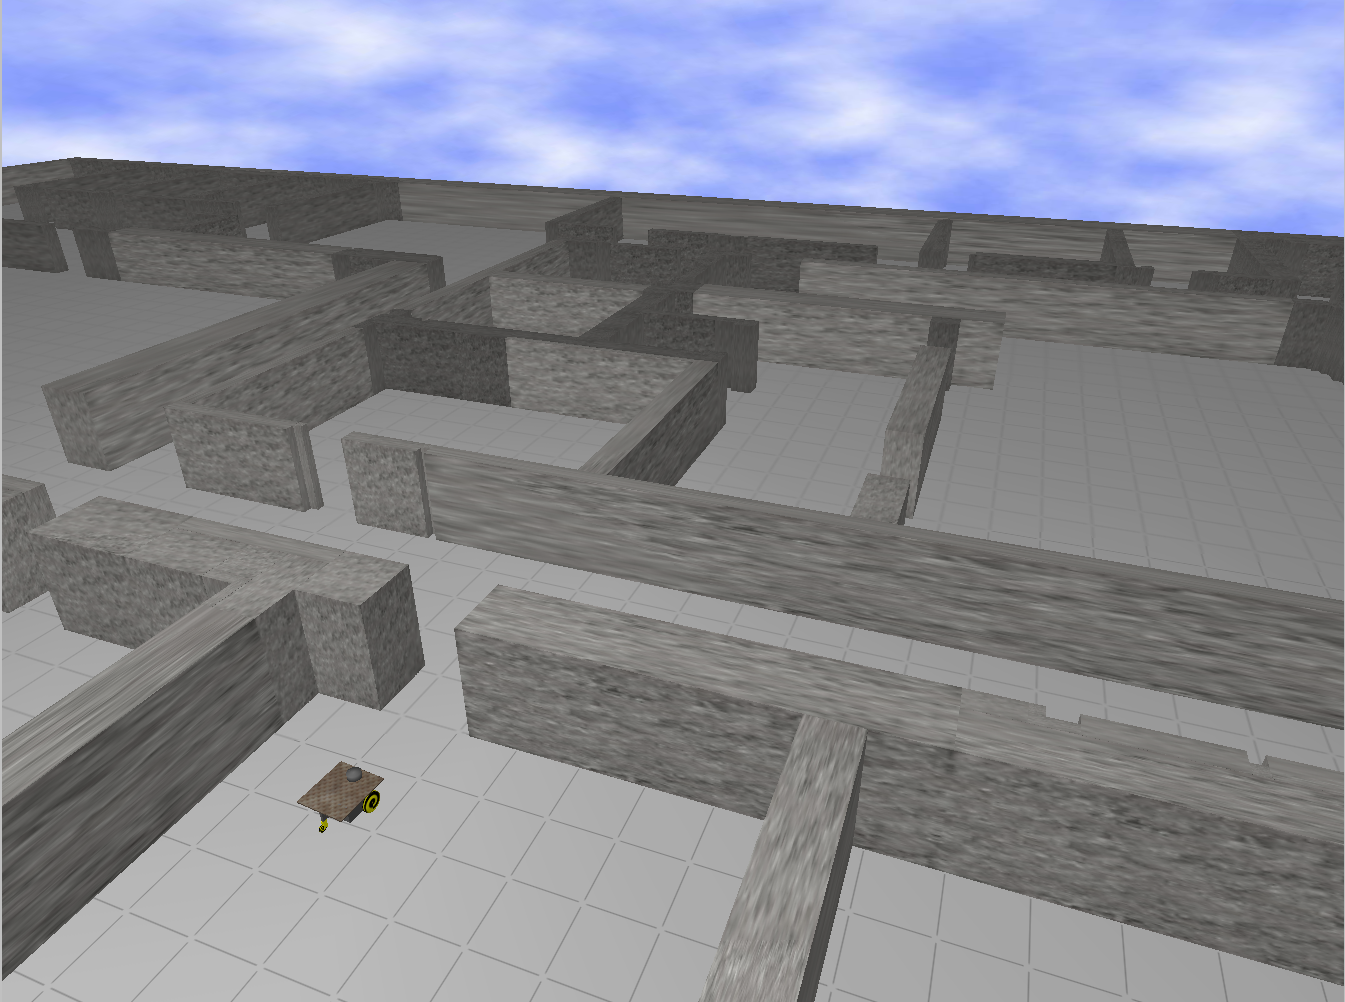
\includegraphics[width=0.8\textwidth]{robot2.png}\\
						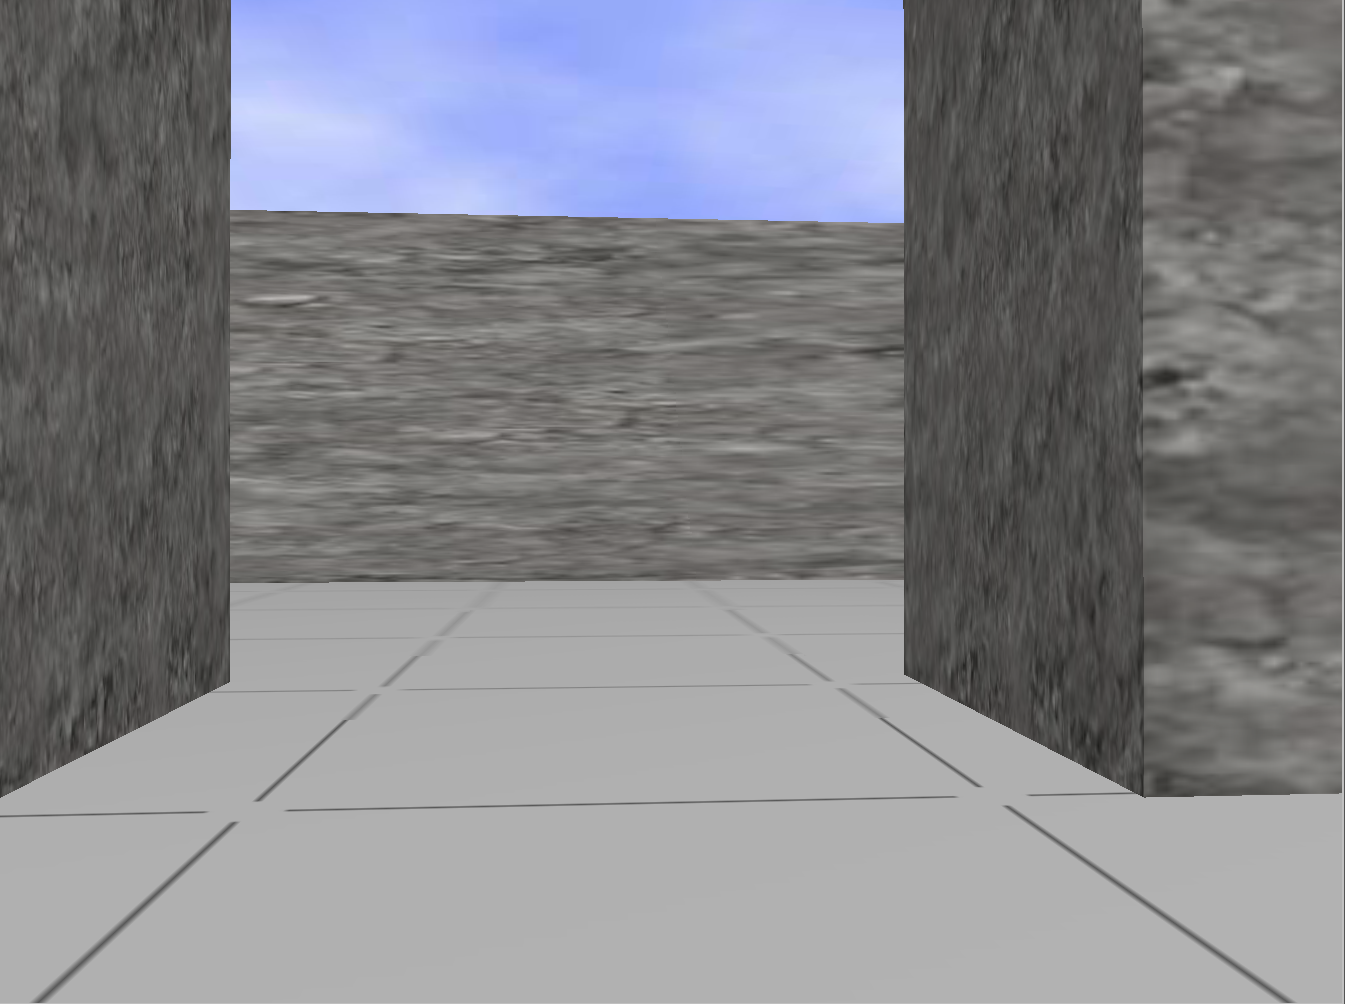
\includegraphics[width=0.8\textwidth]{robot_cam.png}
					\end{center}
				\end{figure}

				\vspace{-0.6cm}
				\scriptsize
				\begin{itemize}
				\item Environment (Top)
				\item Robot's Camera (Bottom)
				\end{itemize}

		\end{columns}

	\end{frame}

%%%%%%%%%%%%%%%%%%%%%%%%%%%%%%%%%%%%%%%%%%%%%%%%%%%%%%%%%%%%%%%%%%%%%%%%%%%%%%%%
\section{Approach}

	\begin{frame}{Approach}

		\begin{columns}[c c]
		
			\column{0.55\textwidth}
			\vspace{-2cm}
			
			\begin{itemize}

			\item Generate populations

			\item Create mutants from populations
				\begin{itemize}
				\item $\epsilon$-greedy selection
				\end{itemize}

			\item For $n$ frames:
				\begin{itemize}
				\item Slice frame
				\item Generate command
				\item Evaluate mutants
				\end{itemize}

			\item Replace
			
			\item Repeat from step 2

			\end{itemize}

%					\begin{algorithmic}
%						\footnotesize	
%						\STATE Generate 8 random populations
%
%						\FOR {50 episodes}
%		
%							\FOR {Each population}
%								\STATE $chosen \gets$ best or random using $\epsilon$-greedy.
%								\STATE $mutant \gets mutate(chosen)$
%							\ENDFOR
%				
%							\FOR {100 images}
%		
%								\STATE Split image into 8 slices
%			
%								\FOR {Each slice}
%									\STATE Evaluate slice with corresponding mutant
%									\STATE $grade \gets grade + abs(desired - output)/100$
%								\ENDFOR
%			
%							\ENDFOR
%
%							\FOR {Each population}		
%								\IF{$grade < worst(population)$}
%									\STATE Replace worst in the population with the mutant.
%								\ENDIF
%							\ENDFOR
%
%						\ENDFOR
%					\end{algorithmic}


			\column{0.5\textwidth}

				\begin{figure}
					\begin{center}
						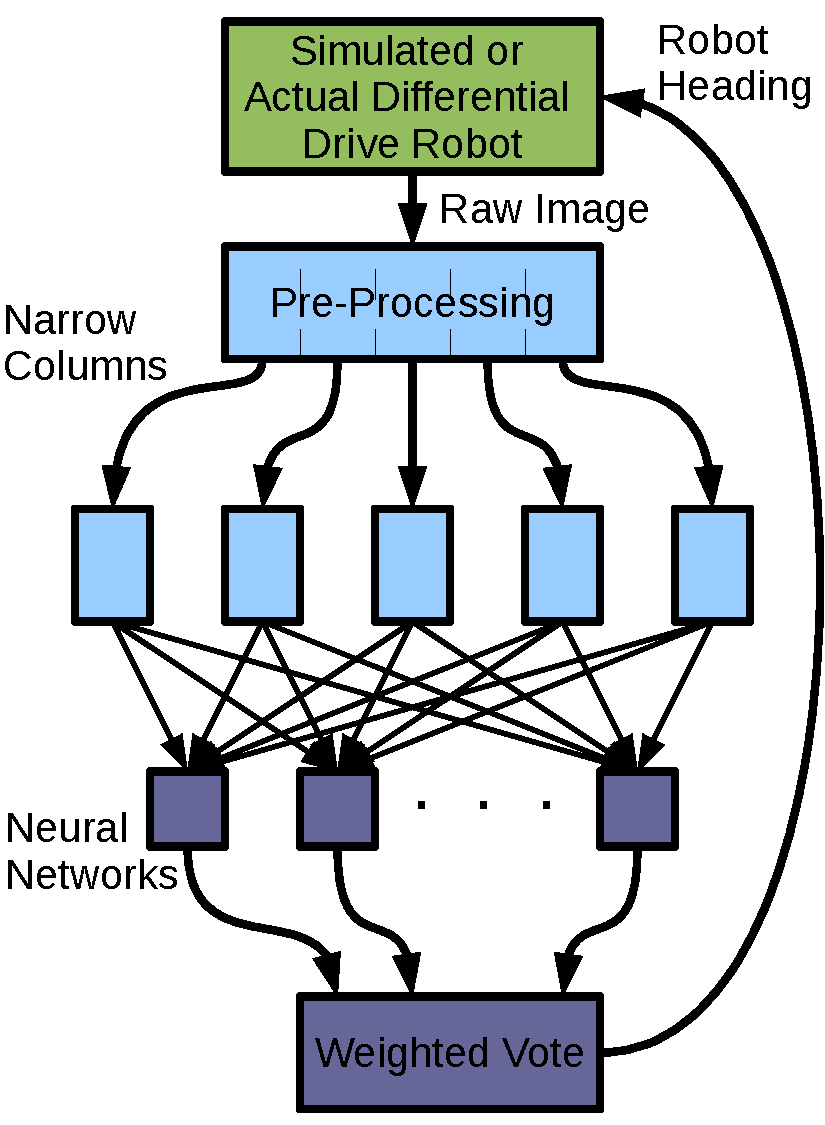
\includegraphics[width=\textwidth]{block_diagram.pdf}
					\end{center}
					\caption{Block diagram.}
					\label{block_diagram}
				\end{figure}

		\end{columns}
	\end{frame}

%%%%%%%%%%%%%%%%%%%%%%%%%%%%%%%%%%%%%%%%%%%%%%%%%%%%%%%%%%%%%%%%%%%%%%%%%%%%%%%%
\section{Experiments}

	\begin{frame}{Experiments}

		\begin{columns}[c c]
		
			\column{0.6\textwidth}

				\begin{itemize}
	
					% something about the number of trials
					%  and specific parameters for tests.
					
					\item Supervised Learning
						\begin{itemize}
						\item Training examples generated by expert driver
						\item Reward based on difference between output and expert command
						\end{itemize}
	
					\item Unsupervised Learning
						\begin{itemize}
						\item Large penalty for bumping walls
						\item Small reward for heading straight
						\end{itemize}
							
				\end{itemize}


			\column{0.4\textwidth}
				\vspace{-0.5cm}
				
				\begin{figure}
					\begin{center}
						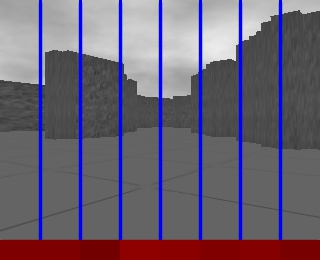
\includegraphics[width=0.8\textwidth]{output_0.jpg}\\
						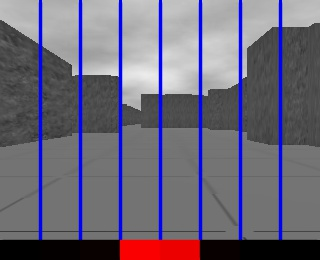
\includegraphics[width=0.8\textwidth]{output_end.jpg}
					\end{center}
				\end{figure}

				\vspace{-0.6cm}
				\scriptsize
				\begin{itemize}
				\item Untrained networks (top)
				\item Trained (bottom)
				\end{itemize}

		\end{columns}


	\end{frame}
	
%%%%%%%%%%%%%%%%%%%%%%%%%%%%%%%%%%%%%%%%%%%%%%%%%%%%%%%%%%%%%%%%%%%%%%%%%%%%%%%%
\section{Results}

	\begin{frame}{Supervised Learning Results}

		\begin{columns}[c c]
		
			\column{0.5\textwidth}
				\begin{itemize}
				\item Offline Learning
					\begin{itemize}
					\item Converges Quickly on Training Data
					\item Easy to Overfit
					\end{itemize}
				\item Online Learning
					\begin{itemize}
						\item Slower, but Still Able to Converge
						\item Learns the Expert as Much as the Environment
					\end{itemize}
				\end{itemize}

			\column{0.5\textwidth}

				\begin{figure}
					\begin{center}
						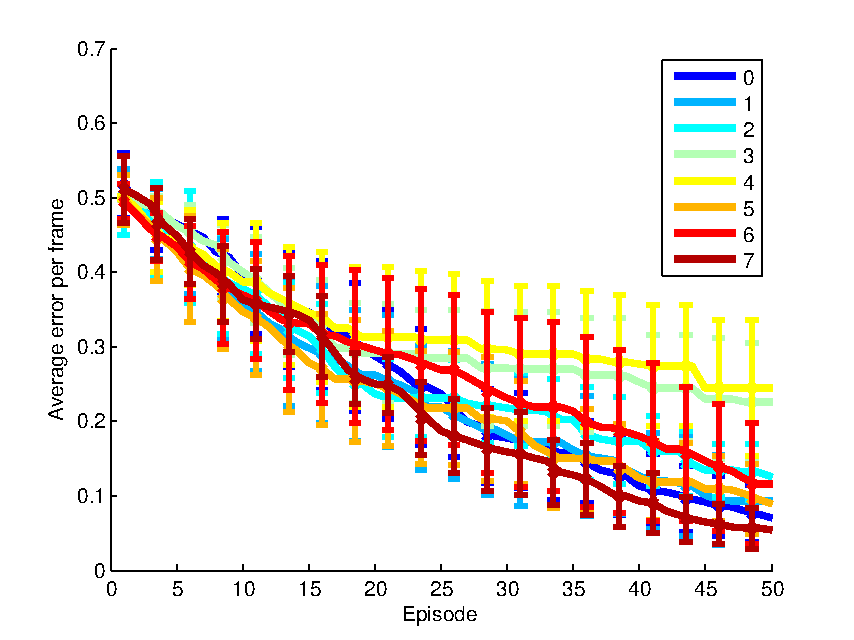
\includegraphics[width=\textwidth]{data.pdf}
					\end{center}
					\label{results}
				\end{figure}

				\begin{itemize}
					\item Neural Network Ensembles Learn Expert Commands.
				\end{itemize}

		\end{columns}

	\end{frame}

	\begin{frame}{Supervised Learning Results}
		\begin{figure}
			\includemovie[poster, text={\small(Overfit...)}]{6cm}{6cm}{overfit.mpg}
		\end{figure}

		\begin{itemize}
			\item Overfitting
			\item Would Not Generalize Well
		\end{itemize}
	\end{frame}

	\begin{frame}{Unsupervised Learning Results}
		%\begin{figure}
		%	\includemovie[poster, text={\small(Overfit...)}]{6cm}{6cm}{overfit.mpg}
		%\end{figure}

		\begin{itemize}
			\item Often Learns to Spin
			\item This Behavior Does a Good Job of Avoiding Obstacles
			\item More Interesting Behaviors Rarely Emerge
		\end{itemize}
	\end{frame}

%%%%%%%%%%%%%%%%%%%%%%%%%%%%%%%%%%%%%%%%%%%%%%%%%%%%%%%%%%%%%%%%%%%%%%%%%%%%%%%%
\section{Conclusions}

	\begin{frame}{Conclusions}

		\begin{columns}[c c]

		\column{0.7\textwidth}

		\begin{itemize}
			\item Supervised Learning
				\begin{itemize}
					\item Many Possible Good Actions
					\item Expert May Not Make Optimal Actions
					\item Difficult to Associate Expert's Actions with the Environment
				\end{itemize}
			\item Unsupervised Learning
				\begin{itemize}
					\item Good Reward Function Difficult
					\item Eventually Discovers Optimal Behaviors
					\item Optimal Behaviors May Not be Desirable
					\item Spinning in Tight Circles
				\end{itemize}
		\end{itemize}

		\column{0.3\textwidth}

			\begin{figure}
				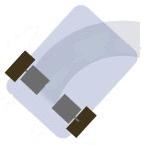
\includegraphics[width=\columnwidth]{differential.jpg}
				\label{diff_drive}
			\end{figure}

		\end{columns}

	\end{frame}

%%%%%%%%%%%%%%%%%%%%%%%%%%%%%%%%%%%%%%%%%%%%%%%%%%%%%%%%%%%%%%%%%%%%%%%%%%%%%%%%

\section{Discussion}

	\begin{frame}{Discussion}

		\begin{columns}[c c]		

		\column{0.6\textwidth}
		
		\begin{itemize}
				\item Learning Currently Limited
				\item Need Global and Differentiable Reward Function
					\begin{itemize}
						\item Difference Rewards
					\end{itemize}
				\item Online Experience Inconsistent
					\begin{itemize}
						\item Restarts
						\item Learn on Repeatable Scenarios
					\end{itemize}
				\item Potential to Combine Supervised and Unsupervised Learning
%					\begin{itemize}
%						\item Supervised Learning Achieves Basic Desired Behavior Easier
%						\item Unsupervised Learning More Likely to Converge to Optimal Behavior
%					\end{itemize}
				\item However, Our Approach Overcomes These Limitations
		\end{itemize}

		\column{0.4\textwidth}

			\begin{figure}
				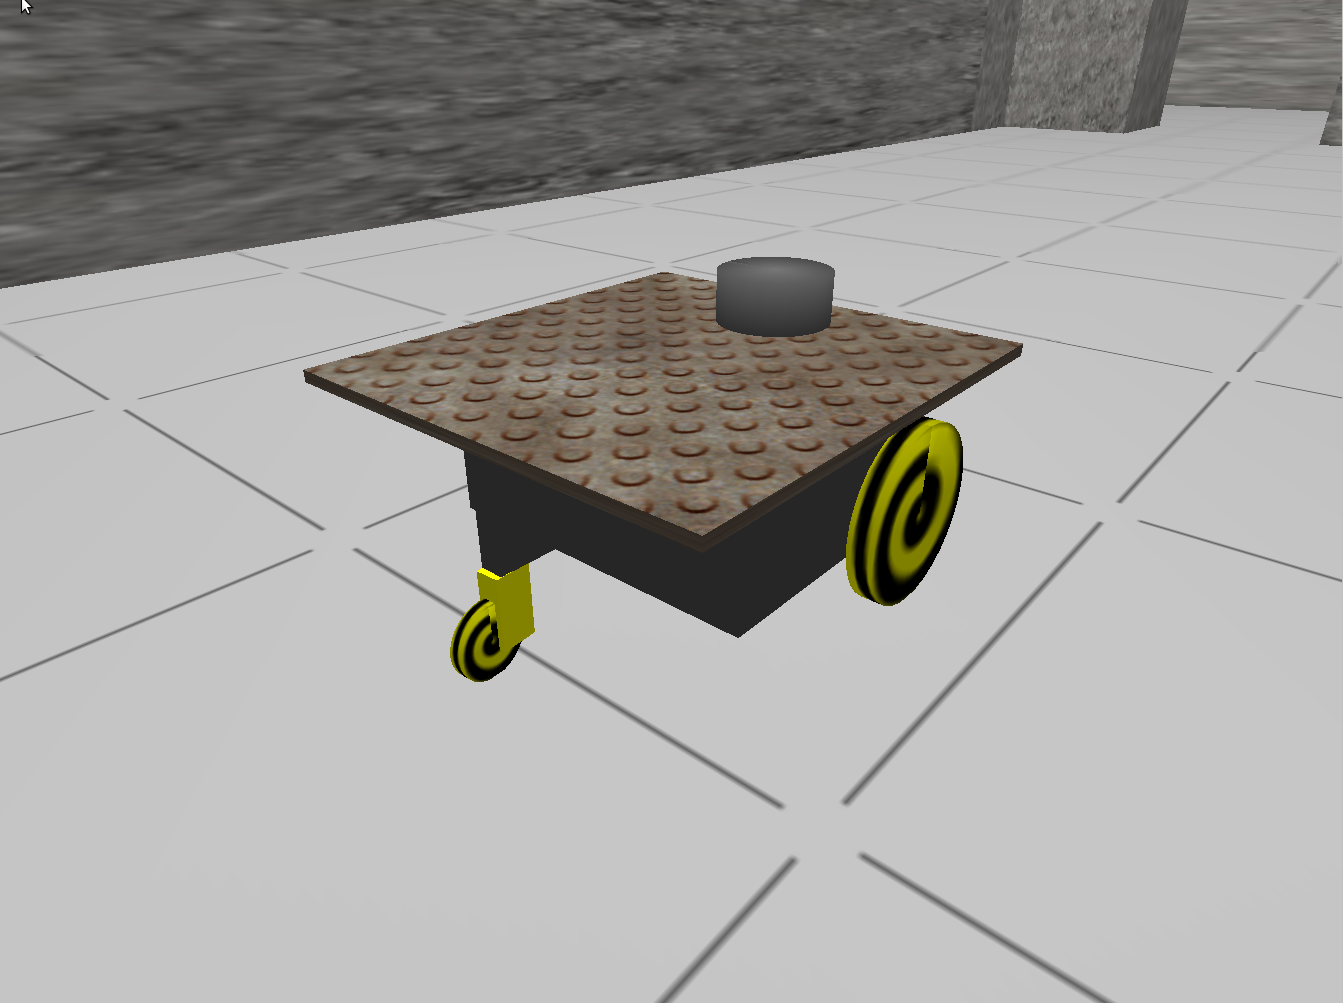
\includegraphics[width=\columnwidth]{robot1.png}
				\label{our_robot}
			\end{figure}

		\end{columns}

	\end{frame}

%%%%%%%%%%%%%%%%%%%%%%%%%%%%%%%%%%%%%%%%%%%%%%%%%%%%%%%%%%%%%%%%%%%%%%%%%%%%%%%%
\section{Future Work}
	\begin{frame}{Future Work}

		\begin{columns}[c c]

			\column{0.6\textwidth}

				\begin{itemize}
					\item Varying Environments
						\begin{itemize}
						\item Colors and Textures
						\item Multi-Agent
						\item Changes in Elevation
						\end{itemize}
					\item Better Reward Functions
						\begin{itemize}
						\item Localized Rewards
						\item Distance Sensor
						\end{itemize}
					\item Higher Level Objectives
						\begin{itemize}
						\item Deliver Packages
						\item Explore Terrain
						\item Avoid Predators
						\end{itemize}
				\end{itemize}

			\column{0.4\textwidth}

				\begin{figure}
					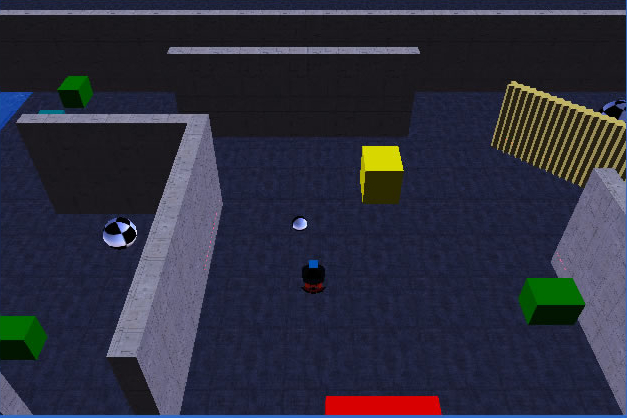
\includegraphics[width=\columnwidth]{SimulatorInitialView.jpg}
					\label{Roomba}
				\end{figure}

				\begin{figure}
					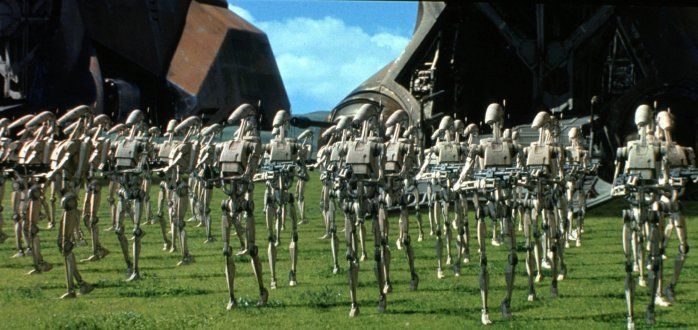
\includegraphics[width=\columnwidth]{sm_eog_droid_army.jpg}
					\label{Roomba}
				\end{figure}

		\end{columns}

	\end{frame}


	\begin{frame}{}
		\vspace{24pt}
		\begin{center}
			\Huge{Thank You!}
		\end{center}
	\end{frame}

%%%%%%%%%%%%%%%%%%%%%%%%%%%%%%%%%%%%%%%%%%%%%%%%%%%%%%%%%%%%%%%%%%%%%%%%%%%%%%%%



%%%%%%%%%%%%%%%%%%%%%%%%%%%%%%%%%%%%%%%%%%%%%%%%%%%%%%%%%%%%%%%%%%%%%%%%%%%%%%%%

%	\frame
%	{
%		\begin{figure}[ht]
%			\includemovie[poster,	text={\small(Loading Video...)}]{6cm}{6cm}{circle.mp4}
%		\end{figure}
%	}

\end{document}

